	\section{Exkurs: Emergenz der Entropie}
	
	\begin{center}
		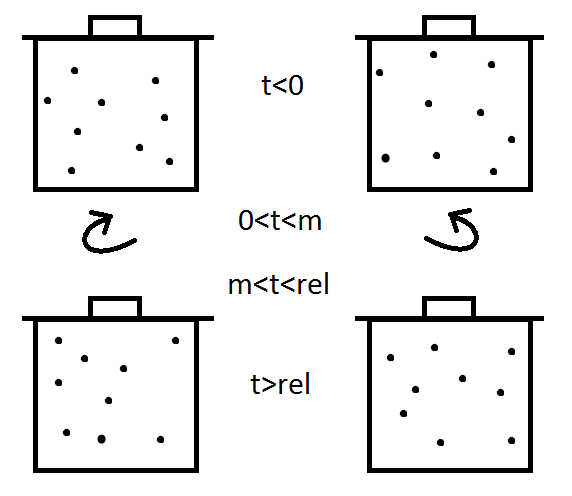
\includegraphics[width=0.6\textwidth]{Abb/Emergenz.png}
	\end{center}%
	Man stelle sich zwei mit Gas gefüllte Behälter in zwei verschiedenen Laboratorien vor. Beide besitzen -innerhalb einer gewissen Fehlertoleranz- die gleichen charakteristischen Zustandsgrößen und lassen sich anhand dieser zum Zeitpunkt $t<0$ nicht unterscheiden. Im Zeitintervall $0<t<m$ werden die beiden Behälter nun in unterschiedliche Richtungen gerührt und sind im folgendem $m>t>rel$ voneinander unterscheidbar. Nach einer gewissen Relaxationszeit $rel$ befinden sich die beiden Gase wieder im Gleichgewicht und sind makroskopisch nicht mehr voneinander zu unterscheiden. Die makroskopische Beschreibung hat das Rühren "vergessen". 

	
\chapter{Grundlegende Konzepte der Statistik und der Wahrscheinlichkeitstheorie}

	\paragraph{klassische Mechanik:}
		Mittelwert, Varianz, Verteilungsfunktionen, Korrelationen ect.
	\paragraph{QM:}
		analoge Bildungen.
		
	\section{Klassische Statistik}
	
	\begin{figure}[H]
		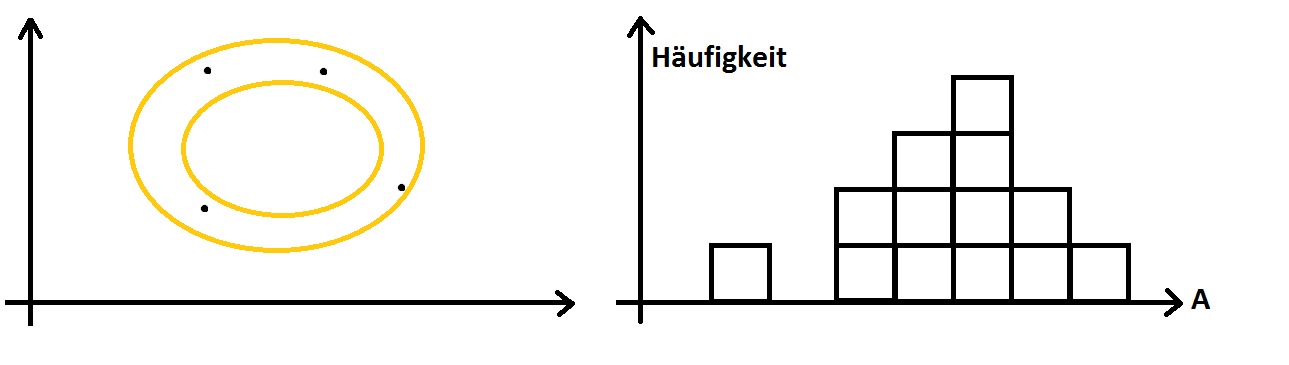
\includegraphics[width=0.9\textwidth]{Abb/abb21.png}
		\caption{Links: bildliche Darstellung der Menge aller Ensemble im 6N-Dimensionelen Raum mit Achsen $p$ und $x$.\\ Rechts: Histogramm (oft $\frac{\text{Häufigkeit}}{\text{Anzahl}}$, so dass dieses normiert ist.)}
		\label{HTT}
	\end{figure}
		
	Aus der Abb. \ref{HTT} folgt intuitiv die Definition des Mittels. Um dieses zu erhalten Summiert man alle Werte $A(p^{(j)},x^{(j)})$ des betrachteten Ensembles $\{p^{(j)},x^{[j]}\}, j=1,...,J $ und Teilt durch die Anzahl der Elemente des selbigen.
	\begin{align*}
		\langle A \rangle = \frac{1}{J} \sum_{j=1}^{J} A(p^{(j)},x^{(j)}) \\
	\end{align*}
	
	\noindent Durch den Übergang zu beliebig genauen Messgenauigkeiten, wird die diskrete Verteilung in Abb. \ref{HTT} zu einer kontinuierlichen Kurve. (Übergang zum Kontinuumslimes.)
	
	\begin{figure}[H]
		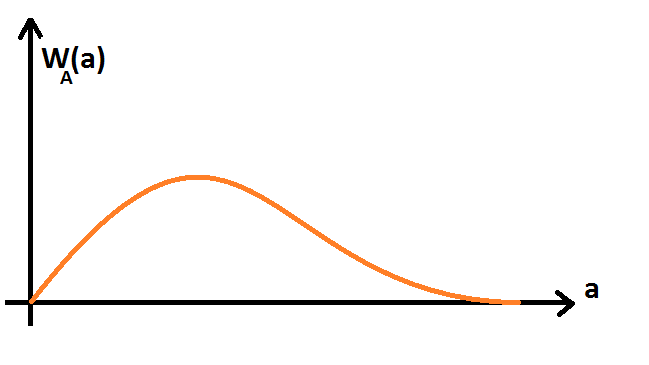
\includegraphics[width=0.9\textwidth]{Abb/abb22.png}
		\caption{Übergang zum "Kontinuumslimes" mit Wahrscheinlichkeit $W_A(a)$.}
	\end{figure}
	\noindent Wie oben ist auch diese Kurve normiert. Die Häufigkeit wird ersetzt durch $W_A(a)$, welche die Wahrscheinlichkeit angibt, für ein gegebenes Ensemble, eine Messgröße $A$ mit dem Wert $a$ zu Messen. 	
	\newline \newline
	Im Folgenden sollen nun noch kurz einige wichtige Begrifflichkeiten aus der Statistik definiert werden.
	
	\paragraph{Varianz:}
	\[\langle [A - \langle A \rangle]^2 \rangle  = \langle A^2 \rangle - \langle A \rangle^2 \]
	\paragraph{Weitere Momente:}\footnote{Definition und mehr auch im Bronstein "Taschenbuch der Mathematik"}
	\[ \langle A^k \rangle = \frac{1}{J} \sum_{j=1}^{J}(A(p^{(j)},x^{(j)}))^k \]
	\paragraph{Phasenraumdichte:}\footnote{$ \delta(p-p^{(j)}) = \delta(p_{1x}-p_{1x}^{(j)}) \cdot \delta(p_{1y}-p_{1y}^{(j)})\cdot ... \cdot \delta(p_{Nz}-p_{Nz}^{(j)})$.}
	\[ \rho (p,x) = \frac{1}{J} \sum_{j=1}^{J} \delta(p-p^{(j)}) \delta(x-x^{(j)}) \]
	
	\noindent Mithilfe der Phasenraumdichte lässt sich jetzt der Mittelwert auch mithilfe eines Integrals beschreiben: 
	\[ \langle A \rangle \int dp^{3N} dx^{3N} \rho (p,x) A(p,x)\]
	
	\subsection{Motivation für die Einführung der Phasenraumdichte:}
	Zum einen erlaubt die Einführung durch Produktbildung die Trennung der Eigenschaften von Beobachtungsgrößen und Ensemble, zum anderen ist dies die mathematische Umsetzung des Übergangs vom mikroskopischen zum makroskopischen (Coarse-Graining). 
	
	
	
	